\subsection*{Behaviour tree}
Behavior tree are a method to organize the decision making of a system, they have find usage particularly in A.I for
video games and chatbot. They can be considered as an extension of finite state machine [1] \marginpar{[1]:paper}. 
Behaviour trees progress during execution in discrete step called tick, at each tick behaviours are executed based on
the structure and the status of the tree. When being ticked and thus executed a behaviour will return a status, that 
represent the result of the behaviour itself, this status can be \textbf{Success}, \textbf{Failure} \textbf{Running}.

The tree is  composed by different type of nodes: 

\begin{itemize}
  \item Behaviour: behaviours are the leaf of the tree, they represent an action that the robot has to perform 
                   to complete the task. One of the key to make behaviour tree flexible and reusable is to make the 
                   behaviours as simple as possible, and build more complex behaviour as composites. Behaviours are
                   represented graphically as rectancgles, as it can be seen in \gumargin{5}{insert image}
  \item Composites: composites are control nodes and they define how a behaviour tree is traversed. This nodes have 
                    $N$ different children which can be both behaviours or composites. When ticked composites nodes
                    execute these children, and change their status based on them and different policies:
                    \begin{itemize}
                      \item Sequence: they execute each children in order until one of them return running or failure, 
                                      or all of them return success.
                                    \begin{figure}[H]
  \centering
  \begin{subfigure}[t]{0.6\textwidth}
      \begin{algorithm}[H]
        $N \gets $ $number$ $of$ $children$ $of$ $the$ $node$\;
        $i \gets 0$\;
        \While{$i < N$}{
            $childStatus$ $\gets$ $tick(child[i])$\\    
        {\If{childStatus == running or\\
              childStatus == failure }{
              \textbf{return} $childStatus$
            }
          }
        }
        \textbf{return} $childStatus$
    \end{algorithm}
    
      \caption{Pseudo code for sequence node}\label{alg:seq}
      % \caption{Lorem ipsum}
  \end{subfigure}%
  ~ 
  \begin{subfigure}[t]{0.3\textwidth}
      \centering
      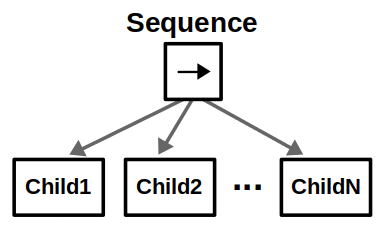
\includegraphics{figs/bt_sequence_node.png}
      \caption{Graphical representation of the node}
      \label{fig:seq}
  \end{subfigure}
  \caption{Caption place holder}
\end{figure}
                      \item Fallback: they execute each children in order unitl one of them return success or all 
                                      of them return failure. They are used for an action that can be achieved in 
                                      different ways
                                      \begin{figure*}[H]
  \centering
  \begin{subfigure}[t]{0.6\textwidth}
      \begin{algorithm}[H]
        % \caption[short]{ASd}
        $N \gets $ $number$ $of$ $children$ $of$ $the$ $node$\;
        $i \gets 0$\;
        \While{$i < N$}{
            $childStatus$ $\gets$ $tick(child[i])$\\    
        {\If{childStatus == running or
              childStatus == failure }{
              \textbf{return} $childStatus$
            }
          }
        }
        \textbf{return} $childStatus$
    \end{algorithm}
    
      \caption{Pseudo code for fallback node}\label{alg:fal}
      % \caption{Lorem ipsum}
  \end{subfigure}%
  ~ 
  \begin{subfigure}[t]{0.3\textwidth}
      \centering
      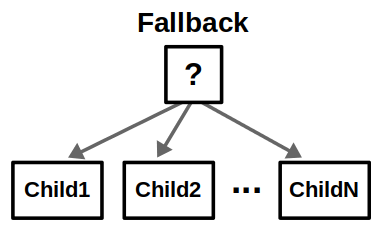
\includegraphics{figs/bt_fallback_node.png}
      \caption{Graphical representation of the node}
      \label{fig:fal}
  \end{subfigure}
  \caption{Caption place holder}
\end{figure*}
                      \item Parallel: they execute each children in a pseudo parallel way, each children is ticked in 
                                      order, the parallel composite will suceed when one or more selected children
                                      suceed
                                      \begin{figure*}[H]
  \centering
  \begin{subfigure}[t]{0.6\textwidth}
      \begin{algorithm}[H]
        $N \gets $ $number$ $of$ $children$ $of$ $the$ $node$\;
        $i \gets 0$\;
        \While{$i < N$}{
            $childStatus$ $\gets$ $tick(child[i])$\\    
        {\If{childStatus == running or\\
              childStatus == failure }{
              \textbf{return} $childStatus$
            }
          }
        }
        \textbf{return} $childStatus$
    \end{algorithm}
    
      \caption{Pseudo code for parallel node}\label{alg:par}
  \end{subfigure}%
  ~ 
  \begin{subfigure}[t]{0.3\textwidth}
      \centering
      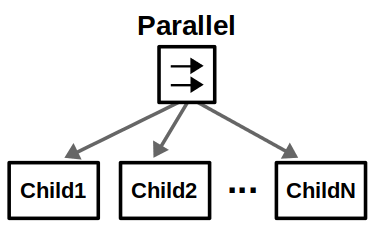
\includegraphics{figs/bt_parallel_node.png}
      \caption{Graphical representation of the node}
      \label{fig:par}
  \end{subfigure}
  \caption{Caption place holder}
\end{figure*}
                    % più esperimenti necessari per questo, un tick dell composite vuol dire un tick per ogni behaviour?
                    % soprattutto se fosse così non c'è differenza tra sequence e parallel, dovrebbe essere che a un tick dell
                    % sequence corrisponde un behaviour per sequence e fallback e multipli per il parallel
\end{itemize} 


The composites nodes are what ensure scalability for behaviour trees, as you can treat composites as complex behaviours,
which can be expanded or reused. This strategy of control also ensure reactivity, especially when the tree implements
parallel nodes, where all the children are execute together.
For all these reasons in latter years behavior tree found new employement in control of robotics arm manipulation task. 

The reactivity and scalability of behaviour tree make them a great candidate for human robot collaboration task as they
make the robot be able to react to a complex agent such as a human. An example of behaviour tree for robot manipulation 
can be seen in figure \gumargin{1}{add figure}

Behaviour tree just follow their structure using the rules of algorithm 1, 2 and 3 \gumargin{2}{add ref to algorithms}
this can lead to problems, eg: in figure \gumargin{3}{add figure} we can see the
example of a behaviour tree that perform a pick and place task, the example is set so that the behaviour tree and the 
operating robot are two distinct part of the system that works together desynchronously. So the behaviour tree will 
communicate with the robot receiving status from it as it runs.

let's analyze the steps the behaviour tree will perform.

\begin{enumerate}
  \item tick the root of the tree, since it is a sequence the node will tick its children until one does return \textbf{running} 
        or \textbf{failure} 
  \item tick the move to grab pose behaviour, which, presumably, will start moving the robot towards the pick location,
        returning \textbf{running}, that will be returned up to the root setting the status of the whole tree
  \item this behaviour will continure returning running for the whole movement of the arm until the robot is in the 
        requested pose, at that point it will return success
  \item since the first child of the sequence returned success the next child will be ticked, it will request the robot
        to close the gripper, 
  \item the robot will close the gripper, and return success, activating the third and last behaviour
  \item the behaviour tree will request the robot to move to the place location
  \item the robot will start moving towards the place location and will communicate to the behaviour tree that it is moiving
        the last action will then be in the \textbf{running} status and that will be returned to the root of the tree
  \item the sequence will start again, from the first child, this will result in a lock state where the behaviour tree
        keep asking the robot to go to the place location and grab the object, effectively never suceeding in the task.
\end{enumerate}

This can be solved in three ways:
\begin{enumerate}
  \item Make the robot blocks the behaviour tree: if the robot instead of returning \textbf{running} while moving would just
        make the behaviour tree wait until it finishes the movement, it would only return \textbf{success} and the end 
        and the problem would not arise. Whereas the solution is simple, and works, doing so would drastically decrease 
        the reactivity of the system, it means that during the whole movement of the robot the behaviour tree would not 
        tick and thus not react to all the changes that could occur in the environment. This is something that we want to avoid
        to ensure the safety of the human operator working with the robot
  \item Store in an external variable the state of the tree: the variable is usually called \textit{blackboard} that
        store the state of the tree's behaviours, this method effectively make the BT works as a Finite State Machine, even if
        this method does solve our problem, it arises the problem of an additional complexity in the management of the 
        system
  \item implement a sequence node with memory: this node is a modified version of the sequence node, that will skip all
        the children that already returned success once
\end{enumerate}

